The label counts also affect how the scores should be read. Phase~3 has only three \emph{PrecedentOverruled} sentences, all from one document, and 284 \emph{Dissent} sentences from two documents. In Phase~4, the 37,387 training rows include 22,067 negative and 15,320 positive outcomes, 5,735 exact duplicate rows and 31,652 case groups. The median document is 13,023 characters long; the 95th percentile is 54,753. Phase~5 has 100 labels, with training support ranging from 272 to 11,730 positives. A case has three labels at the median and eight at the 95th percentile. These differences make grouped validation and per-label calibration important.

\begin{figure}[H]
\centering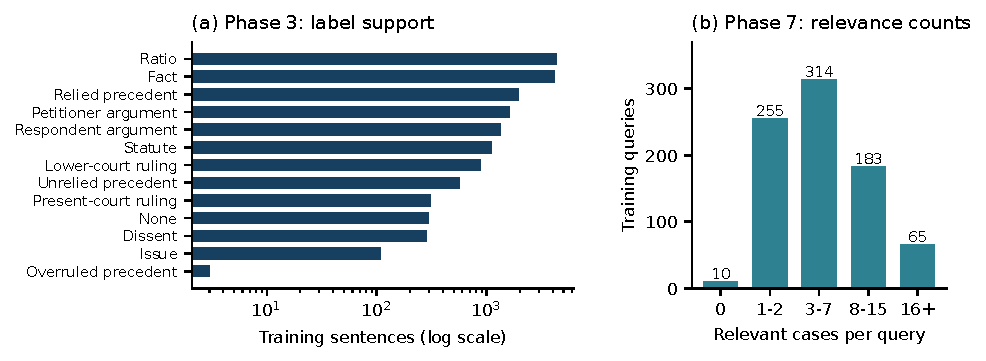
\includegraphics[width=\textwidth]{figures/data_distributions.pdf}
\caption{Aggregate distributions computed from the saved training audits. Rare rhetorical roles concentrate in very few independent documents. Retrieval relevance cardinality spans both sides of the required seven predictions.}
\label{fig:data}
\end{figure}

Long inputs are especially important in the last two tasks. Summarization sources have a median length of 17,911 characters, while references have a median of 638 words and a 95th percentile of 2,010. Retrieval queries have median lengths of 4,508, 4,619.5 and 4,653 words in train, dev and test. They average 6.42 and 8.25 relevant cases in train and dev. Candidate lengths exceed 19,000 words at the 95th percentile in every split. Court and date patterns were not analyzed well enough to justify adding temporal features.

\subsection{Preprocessing}
For NER, the original Unicode text is kept intact so that normalization cannot silently shift character offsets. BPE positions are mapped back to the original character boundaries; 8,241 of 8,393 gold spans match exactly after trimming whitespace. Phase~3 uses the supplied sentence boundaries. Longer cases are split into overlapping chunks, while summarization first selects sentences to fit its source budget. Retrieval uses the same chunk policy for queries and candidates and keeps IDs as strings, preserving leading zeros. Duplicate texts are grouped together during validation.

\section{Approach and Model Evolution}
\subsection{Phase-1 foundation model}
The four foundation models test different attention patterns within the parameter budget~\cite{vaswani2017attention}. Their dimensions are listed in Table~\ref{tab:foundations}, and parameter counts were checked at runtime. Bases~03 and~04 use RoPE and RMSNorm~\cite{su2021roformer,zhang2019rmsnorm}; base~04 also shares key/value heads~\cite{ainslie2023gqa}. Byte-level BPE avoids a fixed word vocabulary for names and legal citations. Bases~01/02 use 32k tokenizers, and bases~03/04 use separate 25k tokenizers.
